\documentclass[10pt, compress]{beamer}

\usetheme{m}

\usepackage{minted}
\usepackage{tikz}
\usetikzlibrary{arrows,decorations.pathmorphing,backgrounds,positioning,fit}

\usemintedstyle{trac}

\title{SYCL presentation}
\subtitle{How to perform stencil computations with SYCL}
\date{\today}
\author{Alexandre Honorat, supervised by Olivier Aumage \& Denis Barthou}
\institute{Inria Bordeaux -- Storm Team}

\begin{document}

\maketitle

\section{Introduction}


\begin{frame}{Stencil computing}

\begin{block}{Stencil example: Jacobi 2D 5-points stencil}
\begin{center}
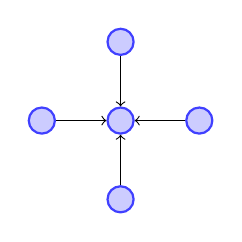
\begin{tikzpicture}
\tikzstyle{place}=[circle,thick,draw=blue!75,fill=blue!20,minimum size=2mm]

\node[place] (p1) at (0,0) {};
\node[place] (p2) at (0,1) {};
\node[place] (p3) at (1,0) {};
\node[place] (p4) at (-1,0) {};
\node[place] (p5) at (0,-1) {};

\draw[->] (p2) to (p1);
\draw[->] (p3) to (p1);
\draw[->] (p4) to (p1);
\draw[->] (p5) to (p1);

\end{tikzpicture}
\end{center}
\end{block}

\begin{block}{High perfromance? $\Rightarrow$ Data reuse}
\end{block}

\begin{block}{Use cases}
\begin{itemize}
\item image processing
\item physics computing (e. g. \texttt{QIRAL})
\end{itemize}
\end{block}

\end{frame}


%%

%\begin{frame}{Qiral overview}

%\begin{block}{A high-level language for physicists}
%\begin{itemize}
%\item they write algorithms in \textbf{\LaTeX} ~(in \texttt{algorithm2e} package)
%\item all agorithms are pure maths (plus control statements)
%\end{itemize}
%\end{block}

%\begin{block}{Automatic parallelization}
%\begin{itemize}
%\item equations rewrritten by \texttt{Maude} in \texttt{C + OpenMP}
%\item result programm automatically generated then compiled
%\end{itemize}
%\end{block}

%\begin{block}{Pitfalls}
%\begin{itemize}
%\item only for CPU %talk about klang
%\item use \texttt{Maude} for some code optimizations
%\end{itemize}
%\end{block}

%\end{frame}

\begin{frame}{SYCL overview}

\begin{block}{New C++ parallelism library}
\begin{itemize}
\item \alert{triSYCL} : prototype working with \texttt{OpenMP}, by \texttt{AMD}.
\item \alert{SYCLONE} : compiler working with \texttt{OpenCL}, by \texttt{CodePlay}. 
\end{itemize}
\end{block}

\begin{block}{Aims}
\begin{itemize}
\item to avoid the burden of wrtting device management code
\item to facilitate kernel launching
\item to hide memory management
\end{itemize}
\end{block}

\end{frame}

\begin{frame}[fragile]{How to use SYCL}

\begin{block}{Workflow}
\begin{enumerate}
\item initialize buffers
\item declare parallel region
\item declare buffer accesors
\item write kernels (\verb!parallel_for!, \verb!parallel_for_workgroup/workitem!)
\item retrieve result by host accessors
\end{enumerate}
\end{block}

\begin{block}{Cool stuff}
\begin{itemize}
\item same notions and compatibily with \texttt{OpenCL}
\item kernel in lambda-functions
\item indexation directly in 1D, 2D and 3D
\end{itemize}
\end{block}

\end{frame}


\begin{frame}[fragile]{Jacobi 2D example code in SYCL}

\begin{minted}[fontsize=\footnotesize]{cpp}
buffer<float,2> ioABuffer(&ioA[0][0], range<2> {M, N});
buffer<float,2> ioBBuffer(&ioB[0][0], range<2> {M, N});
{    
    queue myQueue;
    command_group(myQueue, [&]() {
        accessor<float, 2, access::read>  a(ioABuffer);
        accessor<float, 2, access::write> b(ioBBuffer);
        parallel_for<class KernelCompute>(range<2> {M-2, N-2}, 
                                            id<2> {1, 1},
                                [=] (item<2> it) {
                                id<2> index = it.get_global_id();
                                id<2> id1(range<2> {0,1});
                                id<2> id2(range<2> {1,0});
                                b[index] = a[index] + a[index+id1] + 
                                           a[index+id2] + a[index-id1] 
                                           + a[index-id2];
                                });
    });
}
\end{minted}

\end{frame}


\begin{frame}{Our work}

\begin{block}{Goals}
\begin{enumerate}
\item \large{overlay \texttt{SYCL} with a stencil library}
\item \large{to evaluate \texttt{triSYCL} with a Jacobi code}
\item \large{to make \texttt{triSYCL} use \texttt{StarPU}}
\item \normalsize{\alert{to do:} to test \texttt{SYCLONE} and eventually have \texttt{StarPU} as back-end}
\item \normalsize{\alert{to do:} to make \texttt{QIRAL} use our work on \texttt{SYCL} as back-end}
\end{enumerate}
\end{block}

\end{frame}

%%

\section{Stencil specific library}

\begin{frame}{Overview}

\begin{block}{Aims}
\begin{itemize}
\item facilitate parallelization of stencil;
\item avoid code information redundancy;
\item avoid dynamic information determination.
\end{itemize}
\end{block}

\begin{block}{Means}
\begin{itemize}
\item \texttt{C++14} and especially metaprogramming;
\item parallelization interface \texttt{SYCL}.
\end{itemize}
\end{block}

\begin{block}{Related work}
\texttt{Blitz++} by T. veldhuizen.
\end{block}

\end{frame}


\begin{frame}[fragile]{How to describe and use stencils}

\begin{block}{Coefficients}
Identified by the offset to the current element in each dimension:
\begin{minted}{cpp}
coef_var2D<0, 0> c1; /*or*/ coef_fxd2D<-1, 1> c2(0.2f);
\end{minted}
\end{block}

\begin{block}{Stencils}
Adding two or more coefficients (of same type) creates automatically a stencil:
\begin{minted}{cpp}
auto st = c1+c2+c3+c4+c5;
\end{minted}
\end{block}

\begin{block}{Operation on stencil}
Then you associate input and output to the stencil:
\begin{minted}{cpp}
auto op_work = workload_out << st << workload_in;
\end{minted}
\end{block}

\end{frame}


\begin{frame}[fragile]{Access functions}

\begin{block}{Two sort of functions:}
\begin{enumerate}
\item{to determine coefficients:
\begin{minted}[fontsize=\footnotesize]{cpp}
T (*coefsAccessFun) (int, int, int, int, 
    cl::sycl::accessor<T, 1, cl::sycl::access::read>)
\end{minted}
}
\item{to define the data layout:
\begin{minted}[fontsize=\footnotesize]{cpp}
T (*dataLayoutFun) (int, int, 
    cl::sycl::accessor<T, 2, cl::sycl::access::read>)
\end{minted}
}

\end{enumerate}
\end{block}

\begin{block}{Usage}
\begin{itemize}
\item user-written, in a static manner at the begin of the file
\item{output informations = a buffer + a data layout function
\begin{minted}[fontsize=\footnotesize]{cpp}
output_2D<float, &outputBuffer, &dataLayoutFun> workload_out;
\end{minted}
}
\item{input informations = a buffer + a data layout function\\(+ a coefficients buffer + a coefficients access function)
\begin{minted}[fontsize=\footnotesize]{cpp}
input_var2D<float, &inputBuffer, &coefsBuffer,
            &dataLayoutFun, &coefsAccessFun> workload_in;
\end{minted}
}
\end{itemize}

\end{block}

\end{frame}


\begin{frame}{C++ implementation}

\begin{block}{C++14}
\begin{itemize}
\item \texttt{l-value} references
\item advanced \texttt{metaprogramming} (maybe variadic template)
\item \texttt{auto} keyword (to hide template parameters)
\item \texttt{triSYCL}
\end{itemize}
\end{block}

\begin{block}{Low overhead}
Library methods are higly specialized statically with templates.\\
\alert{Tiling static computation}, enables to optimize regarding to the stencil pattern.
\end{block}

\end{frame}

\begin{frame}{Compute computation range automatically}

\begin{block}{Known variables}
\begin{itemize}
\item the stencil width (statically infered)
\item the data range (got dynamicaly from buffer)
\item tile size (statically computed, see next slide)
\end{itemize}
\end{block}

\begin{block}{Policy in global range}
\begin{itemize}
\item input range = output range
\item ghosts are all non computable elements (borders)
\end{itemize}
\end{block}

\begin{block}{Policy in local range, i. e. in a tile}
\begin{itemize}
\item a workitem = an element to write
\item each workitem load a subset of the minimal domain needed including ghosts
\end{itemize}


\end{block}

\end{frame}


\begin{frame}{Compute tiling size}

\begin{block}{Hidden computation}
The \alert{workgroup size} is not specified by the user, it is automatically computed at compile-time.
\end{block}

\begin{block}{Parameters}
\begin{itemize}
\item the stencil width (infered);
\item the number of arrays involved (infered), and the type of their elements (user defined/infered);
\end{itemize}
\end{block}

\begin{block}{Stop conditions (global constants)}
\begin{itemize}
\item the maximum local memory size;
\item the maximum number of workitems in each dimension.
\end{itemize}
\end{block}

\begin{block}{Algorithm}
Increments the size in each dimension until a condition is false.
\end{block}

\end{frame}

\begin{frame}[fragile]{Future work}

\begin{block}{User operator in coefficient declaration}
Enables to select a specific binary operator for coefficients.
\end{block}

\begin{block}{Stencil cascade}
Several stencils are grouped in one logical operation: the output of a stencil is the input of the next one.
\end{block}

\begin{block}{Stencil agregation}
Several stencils are grouped in one physical operation: all have the same input, several outputs.
\end{block}

\begin{block}{Data layout}
Is selected/adapted automatically, usage of \verb!cl::sycl::storage_object!.
\end{block}

\end{frame}


\section{Example}


\begin{frame}[fragile]{Jacobi 2D example code - initialization}

\begin{minted}[fontsize=\footnotesize]{cpp}
using namespace cl;
//static declaration of accesses functions
float& fdl_out(int a,int b, 
                sycl::accessor<float,2,sycl::access::write> acc) 
                {return acc[a][b];}
float  fdl_in(int a,int b, 
                sycl::accessor<float,2,sycl::access::read> acc) 
                {return acc[a][b];}
float  fac(int a,int b, int c, int d, 
            sycl::accessor<float,1,sycl::access::read> acc) 
                {return MULT_COEF*acc[0];}
float  fac_id(int a,int b, int c, int d, 
                sycl::accessor<float,1,sycl::access::read> acc) 
                {return acc[0];}
// static declaration to use buffer pointers
sycl::buffer<float,2> ioBuffer;
sycl::buffer<float,2> ioABuffer;
sycl::buffer<float,1> ioBBuffer;
\end{minted}

\end{frame}

\begin{frame}[fragile]{Jacobi 2D example code - stencil}

\begin{minted}[fontsize=\footnotesize]{cpp}
// SYCL needs
ioBuffer = sycl::buffer<float,2>(io, sycl::range<2> {M, N});
ioABuffer = sycl::buffer<float,2>(ioA, sycl::range<2> {M, N}); 
ioBBuffer = sycl::buffer<float,1>(ioB, sycl::range<1> {1}); 

// coefficients location
coef_var2D<0, 0> c1;  
coef_var2D<1, 0> c2;
coef_var2D<0, 1> c3;
coef_var2D<-1, 0> c4;
coef_var2D<0, -1> c5;

// opertaion construction for stencil
auto st = c1+c2+c3+c4+c5;
input_var2D<float, &ioABuffer, &ioBBuffer, &fdl_in, &fac> work_in;
output_2D<float, &ioBuffer, &fdl_out> work_out;
auto op_work = work_out << st << work_in;
\end{minted}

\end{frame}

\begin{frame}[fragile]{Jacobi 2D example code - computation}

\begin{minted}[fontsize=\footnotesize]{cpp}
//operation construction for copy
auto st_id = c1.toStencil();
input_var2D<float, &ioBuffer, &ioBBuffer, &fdl_in, &fac_id> copy_in;
output_2D<float, &ioABuffer, &fdl_out> copy_out;
auto op_copy = copy_out << st_id << copy_in;

//kernel launching
queue myQueue;
for (unsigned int i = 0; i < NB_ITER; ++i){      
    op_work.doLocalComputation(myQueue);
    op_copy.doComputation(myQueue);
}
\end{minted}

\end{frame}


%%

\section{Evaluation}

%%

\begin{frame}[fragile]{Different versions}

\begin{block}{Sources (Jacobi 2D)}
\begin{itemize}
\item base (OpenMP \verb!for!, row-major)
\item sycl (OpenMP \verb!for!, row-major)
\item tile (OpenMP \verb!task!, row-major)
\item lint (OpenMP \verb!task!, row-major)
\item lint-rt (OpenMP \verb!task!, contiguous tiles)
\item lint-cd (OpenMP \verb!task!, opposite order for loops)
\item lint-hr (OpenMP \verb!task! + \verb!for!, hierarchical)
\end{itemize}
\end{block}
\end{frame}

\begin{frame}{Different variations}

\begin{block}{Internal policies}
\begin{itemize}
\item vector size 
\item first touch
\item malloc/boost
\item copy with tiles
\end{itemize}
\end{block}

\begin{block}{Compiler}
\begin{itemize}
\item clang++3.6
\item g++4.9.2
\item klang (with starpu-1.2)
\end{itemize}
\end{block}

\end{frame}

\begin{frame}[fragile]{Goals}

\begin{block}{Reuse in tile}
\begin{itemize}
\item L3 must contain local tile
\item L2 must contain workitem vectors
\end{itemize}
\end{block}

\begin{block}{Parameters?}
\begin{itemize}
\item vector size ($128$ elts if \verb!float!)
\item tile size ($64 \times 64$ if \verb!float! and $vec\_size = 128$)
\item $\Rightarrow$ 2 second order equations
\end{itemize}
\end{block}

\end{frame}

\section{Results}

\begin{frame}[fragile]{Measures}

\begin{block}{Tools}
\begin{itemize}
\item \verb!gettimeofday!
\item \verb!PAPI!
\end{itemize}
\end{block}

\begin{block}{Parameters}
\begin{itemize}
\item $2$ runs
\item $3$ iterations
\item $32, 64, 128, 256$ for \verb!vec_size!
\item $32, 64, 128, 256$ for \verb!tile_size! (in both dimensions)
\item $514$ for the global size (in both dimensions)
\end{itemize}
\end{block}

\end{frame}

\begin{frame}{On fourmi}
Good
\end{frame}

\begin{frame}{On minotaure}
Bad
\end{frame}

%%

\section{Conclusion}

\begin{frame}{Conclusion}

\begin{block}{Improvements}
To have performance on many-core machines (e. g. \texttt{minotaure}, \texttt{mistral})
\end{block}

\begin{block}{Work to do}
To complete and integrate the stencil specific library, test on real codes
\end{block}

\end{frame}

\plain{}{Questions}

\end{document}
